\vssub
\subsection{~波系的空间和时间追踪} \label{sub:num_track}
\conthead{IFP Swan}{Van der Westhuysen, Hanson, Devaliere}

\noindent
上述谱分区过程在谱空间中进行，并在每个地理网格点上独立完成。因此，识别出的分区在地理空间和时间上并不具有连贯性。按照 \cite{art:VMH97}、\cite{art:HP01} 和 \cite{pro:DHL09}，因此需要应用一个空间相关步骤。该步骤通过从计算域内某个任意点（通常为中心）开始向外运行的螺旋实现。图~\ref{fig:wavetrack} 给出了一个在含陆地区域的近岸规则计算网格上追踪螺旋的示例。在螺旋起点（位置~1），每个谱分区都被赋予一个初始系统索引。随后沿螺旋向外移动，对每个后续地理位置（2、3、4，等等）确定空间相关。在每个新的地理位置，将其每个谱分区的峰值周期 $T_\mathrm{p}$、峰值方向 $\theta_\mathrm{p}$ 和有效波高 $H_\mathrm{m0}$，与此前已分配给系统 $i$ 的相邻地理网格点处对应参数的空间平均值
$\tilde{T}^\mathrm{n}_{\mathrm{p},i}$、
$\tilde{\theta}^\mathrm{n}_{\mathrm{p},i}$ 和
$\tilde{H}^\mathrm{n}_{\mathrm{m0},i}$（以上标
$\mathrm{n}$ 表示）进行相关。当前网格点的分区被分配给使以下拟合优度（GoF）函数最小的相邻系统 $i$：

\begin{figure} \begin{center}
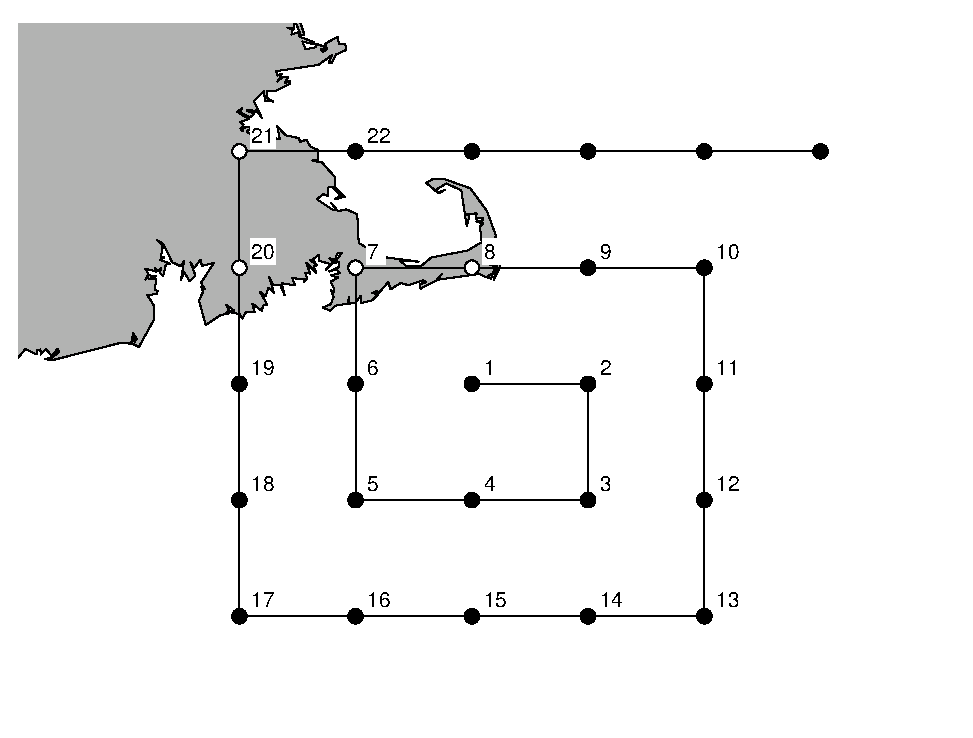
\epsfig{file=./num/wavetrack.eps,width=3.5in}
\caption{含陆地（阴影）的近岸规则计算网格上的追踪螺旋示例。黑点表示活动网格点，白点表示非活动（干）网格点。}
         \label{fig:wavetrack} \botline
\end{center}
\end{figure}

\begin{equation}
    GoF_{i} = {\left( \frac{T_\mathrm{p} - \tilde{T}^\mathrm{n}_{\mathrm{p},i}}{\Delta T_\mathrm{n}} \right)}^2 + 
                     {\left( \frac{\theta_\mathrm{p} - \tilde{\theta}^\mathrm{n}_{\mathrm{p},i}}{\Delta\theta_\mathrm{n}} \right)}^2 +
                     {\left( \frac{H_\mathrm{m0} - \tilde{H}^\mathrm{n}_{\mathrm{m0},i}}{\Delta H_\mathrm{n}} \right)}^2\ \ ,
\label{eq:grdgof}
\end{equation} 

\noindent
其中 $\Delta T_\mathrm{n}$、$\Delta\theta_\mathrm{n}$ 和 $\Delta
H_\mathrm{n}$ 是合并判据 \citep{art:WHD13}。若对于最接近匹配，式~(\ref{eq:grdgof}) 右端前两项中任一项超过 1，则认为差异过大，并将一个新的波系分配给该分区。这里，相邻点搜索范围设为 1，因此最多可找到四个此前已关联的相邻点（例如位置 15 会有此前处理过的相邻点 3、4、5 和 14）。在某些情况下，需要迭代合并。

下一步是在时间上对这些波系进行相关。当前时间层 $t$ 的每个系统 $i$ 与上一时间层 $(t-1)$ 的系统 $j$ 中最接近的匹配相关联。该过程中考虑波系的三个特征，即：(i) 系统内的空间平均峰值波周期 $\tilde{T}^\mathrm{s}_{\mathrm{p},t,i}$，其中
$\mathrm{s}$ 表示系统平均；(ii) 空间平均峰值波向
$\tilde{\theta}^\mathrm{s}_{\mathrm{p},t,i}$；以及 (iii) 两个系统在地理空间中重叠的网格点数 $\cap_{i,j}$。这些特征组合形成以下 GoF 函数：

\begin{equation}
    GoF_{i,j} = {\left( \frac{\tilde{T}^\mathrm{s}_{\mathrm{p},t,i} - \tilde{T}^\mathrm{s}_{\mathrm{p},t-1,j}}{\Delta T_\mathrm{s}} \right)}^2 + 
                       {\left( \frac{\tilde{\theta}^\mathrm{s}_{\mathrm{p},t,i} - \tilde{\theta}^\mathrm{s}_{\mathrm{p},t-1,j}}{\Delta\theta_\mathrm{s}} \right)}^2 +
                       {\left( \frac{N_{t-1,j} - \cap_{i,j}}{0.5N_{t-1,j}} \right)}^2\ \ ,
\label{eq:timegof}
\end{equation} 

\noindent
其中 $\Delta T_\mathrm{s}$ 和 $\Delta\theta_\mathrm{s}$ 是合并判据，$N$ 是一个系统中的网格点总数，见 \cite{art:WHD13}。为使追踪过程聚焦于波场中的高能区域，每个系统的空间平均周期和峰值方向值都按有效波高的平方加权。当前时间层 $t$ 的系统 $i$ 被分配给上一时间层 $(t-1)$ 中使式~(\ref{eq:timegof}) 最小的系统 $j$。若对于使式~(\ref{eq:timegof}) 最小的系统，式~(\ref{eq:timegof}) 右端三项中任一项超过 1，则分配一个新的系统编号。对最后一项而言，这意味着最小空间重叠要求，此处任意设为 50\%。该项主要影响盆地尺度区域，因为此类区域中的系统通常小于计算区域。为提高稳健性，识别出的系统细节会保存五个时间层，之后释放系统关联。
